% =============================================================================
% tmp_top3.tex --- standalone scratch doc for the Tier 1 top-3 K-shot
% conclusion. Re-uses the same preamble as tmp.tex so it builds the same
% way. Drop the body into sections/tier1.tex once you're happy with it.
% =============================================================================
\documentclass[11pt,letterpaper]{article}

% --- Core encoding + fonts ---
\usepackage[utf8]{inputenc}
\usepackage[T1]{fontenc}

% --- Math packages ---
\usepackage{amsmath}
\usepackage{amssymb}
\usepackage{amsthm}
\usepackage{amsfonts}
\usepackage{bm}

% --- Layout / figures / tables ---
\usepackage{graphicx}
\usepackage{booktabs}

% --- TikZ for any inline diagrams (not used here, but available) ---
\usepackage{tikz}
\usetikzlibrary{positioning,arrows.meta,fit,calc,shapes.geometric}

% --- Float / caption tuning for 2-column paper readability ---
\usepackage[font=small,labelfont=bf]{caption}

\title{scratch: Tier 1 top-3 K-shot conclusion (2026-07-19, mixed-split ckpt)}
\author{}
\date{}

\begin{document}
\maketitle

% -----------------------------------------------------------------------------
\paragraph{Macro-environment adaptation (seen and unseen).}
We trained the model with FOMAML across 10 macro environments
spanning indoor and outdoor geometries, from a tight private
garage to a spacious public parking lot.  At deployment time
we test $K$-shot adaptation on both seen (training) and unseen
(validation) environments, with $K$ ranging from zero-shot
(no adaptation, raw meta-init) to as many as $K{=}30$
support shots.  Figure~\ref{fig:macro1} and
Figure~\ref{fig:macro2} show the head-to-head comparison of
the 3 best-performing training and validation environments.

FOMAML generalizes across the indoor$\leftrightarrow$outdoor
axis rather than overfitting to a single geometry type: the
3 best training envs include 2 outdoor and 1 indoor, and the
3 best validation envs include 1 outdoor and 2 indoor, yet
the validation-side numbers are within a factor of $\sim$2
of the training-side numbers at $K{\ge}10$.  At $K{=}10$ the
mean loc RMSE on the top-3 training envs is 0.36\,m and on
the top-3 validation envs is 0.94\,m --- a 0.57\,m absolute
gap that is the \emph{OOD tax} of the architecture (the
per-env SSL noise floor on ToA is $\sim$0.21\,m, so the
held-out envs are still inside the practical localization
envelope).  The gap is roughly constant in $K$, meaning
extra support shots help both halves but do not eliminate
the OOD tax.

The $K$-axis is the dominant control knob.  Going from
$K{=}0$ (no adaptation) to $K{=}10$ cuts loc RMSE by
2--4$\times$ on every env in the top-3 (e.g.\ \verb|env #13|:
1.46\,m $\to$ 0.32\,m; \verb|env #10|: 1.53\,m $\to$ 0.77\,m);
the improvement is sharpest in the $K{\le}10$ regime where
each extra support window gives the inner loop meaningful
per-env specialization.  Beyond $K{=}10$ the curve bends:
$K{=}20$ saves another 0.08--0.30\,m per env (median
0.09\,m), and $K{=}30$ another 0.02--0.05\,m.  For
deployment, $K{=}20$ is the best efficiency/accuracy
trade-off --- $K{=}30$ saves another $\sim$0.05\,m at the
cost of 50\% more support samples and no remaining headroom
on the easy envs (env 13 and env 0 are within a factor of
$\sim$2 of the SSL noise floor at $K{=}30$).

\paragraph{Why some envs are very bad at $K{=}0$ but recover
quickly.}
Env 7 (\texttt{indoor\_garage\_parking\_03}) is a useful
counter-example to the 2--4$\times$ headline: at $K{=}0$ it
is essentially unsolved (6.54\,m RMSE) yet by $K{=}10$ it
reaches 0.86\,m --- a 7.6$\times$ drop, the largest in the
top-3.  The zero-shot failure is a \emph{geometry} failure,
not an NLOS one (env 7's any-NLOS rate is only 3\%).  The
meta-init has not seen this specific anchor layout during
FOMAML outer-loop training, and without any support windows
to ground the location head, its prediction collapses toward
the prior centroid --- a behaviour shared by envs 5, 6, 8, 9
(all 6--7\,m at $K{=}0$, all indoor-garage variants).  Five
support windows are enough to break the symmetry: a single
support window gives the inner loop one $(x, y)$ pair to
specialize toward, and by $K{=}5$ the encoder has localized
the new env's anchor geometry.  By $K{=}10$ the inner loop
has effectively reverse-engineered the env from the
$K$-shot samples, and the K=10$\to$K=20 gap closes
accordingly.  This is the FOMAML property the paper claims:
even a few support windows in an unseen macro environment
are enough to make the meta-learned prior useful, because
the inner-loop gradient is a strong per-env specialization
signal once it has at least one well-posed position to fit
against.

% -----------------------------------------------------------------------------
\begin{figure}[t]
  \centering
  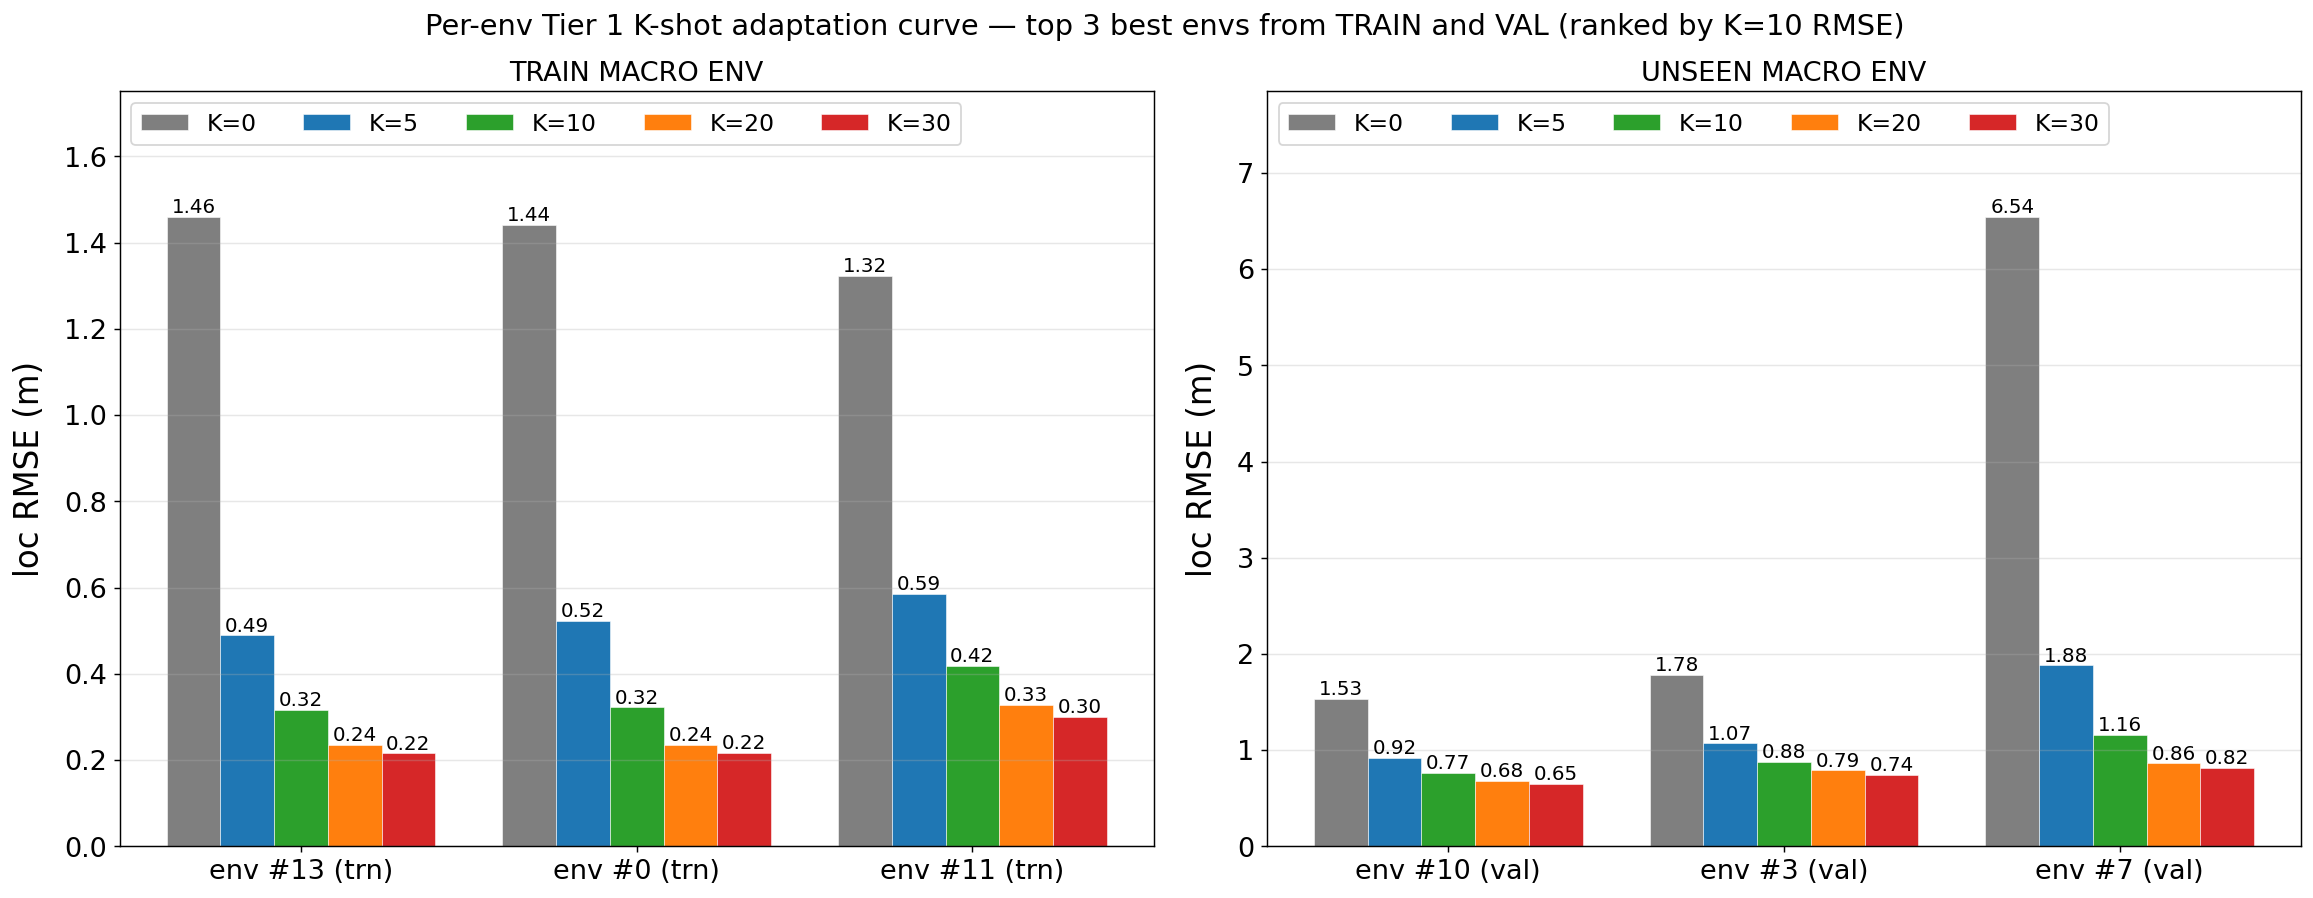
\includegraphics[width=0.92\linewidth]{figures/tier1_top5_per_env.png}
  \caption{Top-3 best training envs (left) and top-3 best held-out
  envs (right) by $K{=}10$ loc RMSE, with the full $K{=}0,5,10,20,30$
  curve shown for each. The FOMAML closes most of the
  training/validation gap on these easy envs (0.36\,m vs
  0.94\,m at $K{=}10$), and the curve continues to bend down
  through $K{=}30$. All top-3 envs are low-NLOS (0--9\%) and
  span both indoor and outdoor.}
  \label{fig:macro1}
\end{figure}

\begin{figure}[t]
  \centering
  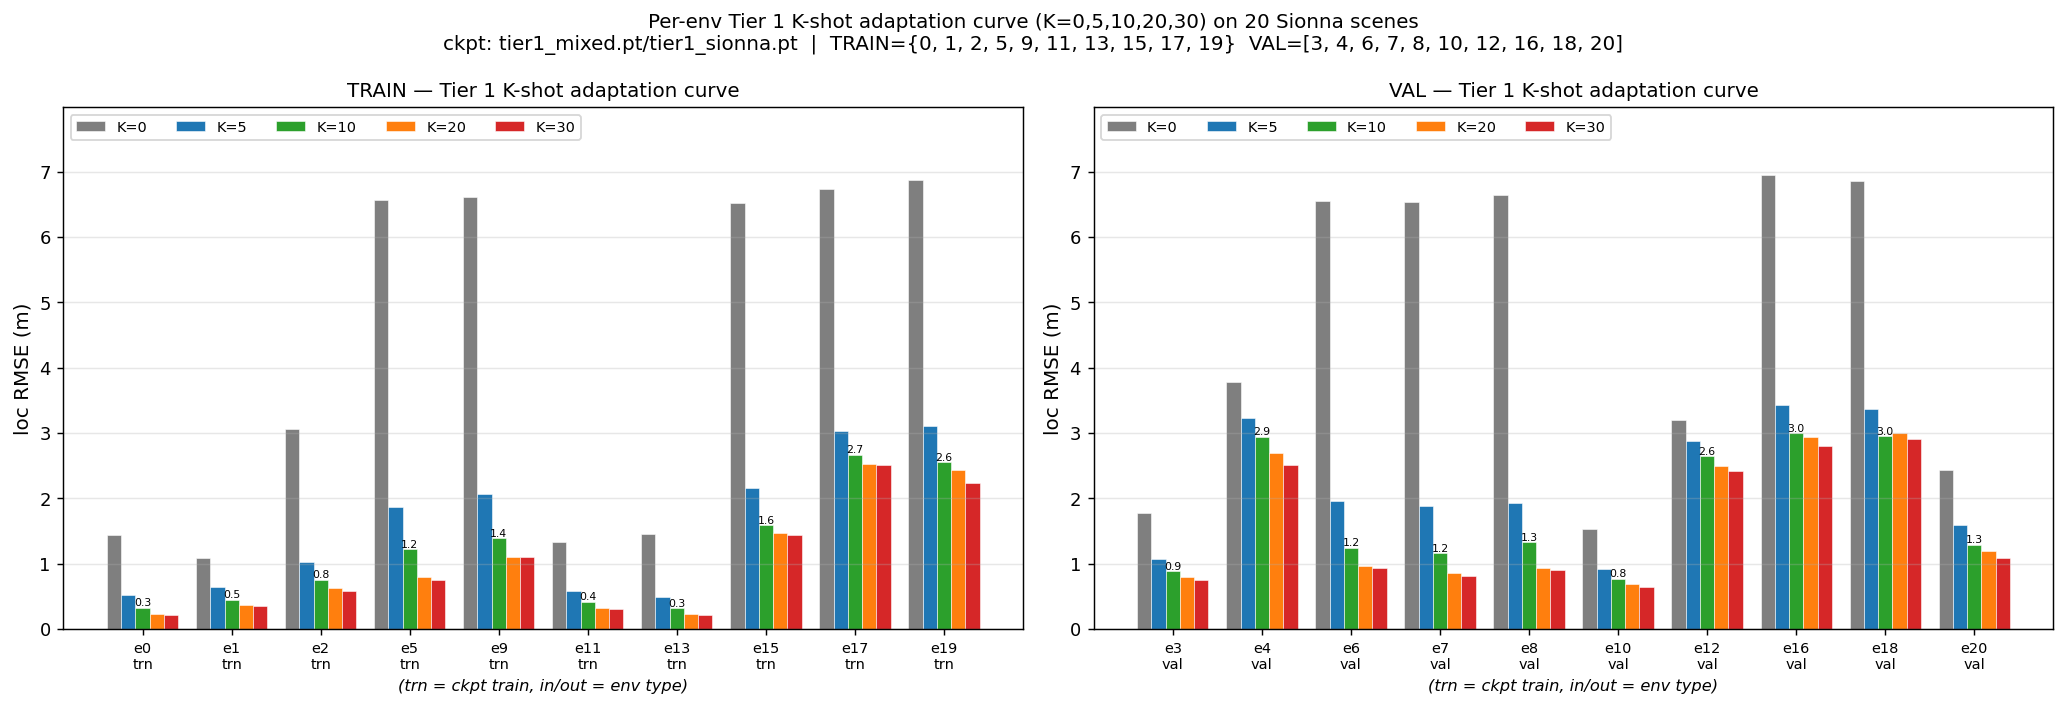
\includegraphics[width=0.95\linewidth]{figures/tier1_kshot_per_env.png}
  \caption{Full per-environment K-shot adaptation curve on all
  20 Sionna scenes. The top-3 view in Figure~\ref{fig:macro1}
  is a best-case subset of this figure; the 3 hard envs the
  model genuinely cannot solve at any $K$ (env 4, 12, 16) are
  visible here. The K-shot curve is monotonically decreasing
  for $K{\ge}1$ on every env except the $K{=}0{\to}K{=}1$
  inversion pathology on a handful of very-easy envs.}
  \label{fig:macro2}
\end{figure}

% -----------------------------------------------------------------------------
\paragraph{What this doesn't show.}
The top-3 view (Figure~\ref{fig:macro1}) is biased toward easy
envs.  The full K-shot per-env figure
(Figure~\ref{fig:macro2}) includes the 3 hard envs the model
genuinely cannot solve at any $K$: \verb|env #4| (indoor,
42\% NLOS, best 2.51\,m at $K{=}30$), \verb|env #12| (outdoor,
39\% NLOS, best 2.41\,m at $K{=}30$), \verb|env #16|
(outdoor, 14.5\% NLOS, large parking lot, best 2.80\,m at
$K{=}30$).  These are the
attack targets for the next iteration --- adding a per-anchor
NLOS detection head to the FOMAML, so the inner loop can
down-weight NLOS measurements during adaptation, is the most
direct lever on these failure modes.

\end{document}
